%% beamer packages
% other themes: AnnArbor, Antibes, Bergen, Berkeley, Berlin, Boadilla, boxes, 
% CambridgeUS, Darmstadt, Dresden, Frankfurt, Goettingen, Hannover, Ilmenau,
%JuanLesPins, Luebeck, Madrid, Malmoe, Marburg, Montpellier, PaloAlto,
%Pittsburgh, Rochester, Singapore, Szeged, Warsaw
% other colors: albatross, beaver, crane, default, dolphin, dove, fly, lily, 
%orchid, rose, seagull, seahorse, sidebartab, structure, whale, wolverine,
%beetle

%\documentclass[xcolor=dvipsnames]{beamer}
\documentclass[table,dvipsnames]{beamer}
\usepackage{beamerthemesplit}
\usepackage{bm,amsmath,marvosym}
\usepackage{listings,color}%xcolor
\usepackage[ngerman]{babel}
\usepackage{natbib}
\usepackage[utf8]{inputenc}
\definecolor{shadecolor}{rgb}{.9, .9, .9}
\definecolor{darkblue}{rgb}{0.0,0.0,0.5}
\definecolor{myorange}{cmyk}{0,0.7,1,0}
%\definecolor{mypurple}{cmyk}{0.5,1.0,0,0.2}
\definecolor{mypurple}{cmyk}{0.3, 0.9, 0.0, 0.2}

% make a checkmark
\usepackage{tikz}
\def\checkmark{\tikz\fill[scale=0.4](0,.35) -- (.25,0) -- (1,.7) -- (.25,.15) -- cycle;} 

% math stuff
\newcommand{\argmin}{\operatornamewithlimits{argmin}}

\lstnewenvironment{code}{
    \lstset{backgroundcolor=\color{shadecolor},
        showstringspaces=false,
        language=python,
        frame=single,
        framerule=0pt,
        keepspaces=true,
        breaklines=true,
        basicstyle=\ttfamily,
        keywordstyle=\bfseries,
        basicstyle=\ttfamily\scriptsize,
        keywordstyle=\color{blue}\ttfamily,
        stringstyle=\color{red}\ttfamily,
        commentstyle=\color{green}\ttfamily,
        columns=fullflexible
    }
}{}

\lstnewenvironment{codeout}{
    \lstset{backgroundcolor=\color{shadecolor},
        frame=single,
        framerule=0pt,
        breaklines=true,
        basicstyle=\ttfamily\scriptsize,
        columns=fullflexible
    }
}{}

\hypersetup{colorlinks = true, linkcolor=darkblue, citecolor=darkblue,urlcolor=darkblue}
\hypersetup{pdfauthor={A. Richards}, pdftitle={Logistic Regression}}

\newcommand{\rd}{\textcolor{red}}
\newcommand{\grn}{\textcolor{green}}
\newcommand{\keywd}{\textcolor{myorange}}
\newcommand{\highlt}{\textcolor{darkblue}}
\newcommand{\norm}[1]{\left\lVert#1\right\rVert}
\def\ci{\perp\!\!\!\perp}
% set beamer theme and color
\usetheme{Frankfurt}
%\usetheme{Berkeley}
\usecolortheme{dolphin}
%\usecolortheme{seagull}
%\setbeamertemplate{blocks}[rounded][shadow=true]

\title[Optimization]{Logistic Regression}
\author[AJR]{Adam Richards}
\institute{Galvanize, Inc}
\date[\today]{Last updated: \today}

%%%%%%%%%%%%%%%%%%%%%%%%%%%%%%%%%%%%%%%%%%%%%%%%%%%%%%%%%%%%%%%%%%%%%%%%%%%%%%%
\begin{document}
\frame{\titlepage}
%%%%%%%%%%%%%%%%%%%%%%%%%%%%%%%%%%%%%%%%%%%%%%%%%%%%%%%%%%%%%%%%%%%%%%%%%%%%%%%
\frame{
\footnotesize
\tableofcontents
\normalsize
}

%%%%%%%%%%%%%%%%%%%%%%%%%%%%%%%%%%%%%%%%%%%%%%%%%%%%%%%%%%%%%%%%%%%%%%%%%%%%%%%
\section{Review}
\subsection{}
%%%%%%%%%%%%%%%%%%%%%%%%%%%%%%%%%%%%%%%%%%%%%%%%%%%%%%%%%%%%%%%%%%%%%%%%%%%%%%%
\frame{   
\frametitle{Objectives}
\begin{block}{}
 \begin{itemize}
  \item Review
  \item The sigmoid function
  \item Logistic Regression
  \item Validation / Confusion Matrix
  \item ROC Curve
 \end{itemize}
\end{block}
}

%%%%%%%%%%%%%%%%%%%%%%%%%%%%%%%%%%%%%%%%%%%%%%%%%%%%%%%%%%%%%%%%%%%%%%%%%%%%%%
% one advantage of the bayesian approach is that overfitting is avoided because the effective number of parameter adopts
% w^{T} is a row vector
% w_{0} is often ommited from the regularizer because it causes the results to depend on the choice of origin for the target variable

\begin{frame}
\frametitle{Review}
\footnotesize

\begin{itemize}
 \item \highlt{Motivation} -
 recall that the least squares approach to finding model parameters represents a specific case of maximum likelihood and overfitting is a general property of maximum likelihood estimation (MLE)

 \item \highlt{So what again is regularization?}
 \visible<2->{ - technique to control overfitting by introducing an a penalty term over the error function to discourage coefficients from reaching large values
 
 \begin{equation}
  \widetilde{E}(\textbf{w}) = \sum^{N}_{n=1} \left\{ y(x_{n},\textbf{w}) - t_{n} \right\}^{2} + \lambda \norm{\mathbf{w}}^{2}   
 \end{equation}

 where 
 \begin{equation}
 \norm{\mathbf{w}}^{2} = \bm{w}^{T} \bm{w} = w_{0}^{2} + w^{2}_{1} \ldots w_{n}^{2} 
\end{equation}
 }
\end{itemize}

 \visible<2->{
Note that $\lambda$ governs the relative importance of the regularization term compared with the SSE term
}

\begin{flushleft}
 \tiny{See pages 5-11 in \citep{Bishop06}}
\end{flushleft}
\end{frame}


%%%%%%%%%%%%%%%%%%%%%%%%%%%%%%%%%%%%%%%%%%%%%%%%%%%%%%%%%%%%%%%%%%%%%%%%%%%%%%
\begin{frame}
\frametitle{More on shrinkage methods}
\scriptsize
\begin{itemize}
 \item \highlt{Why do we use the term shrinkage?}
 \visible<2->{Regularization is also referred to as shrinkage because it reduced the values of the coefficients}
 
 \item \highlt{Lasso Regression?} 
 \visible<3->{
  \begin{equation}
  \hat{\mathbf{w}}^{\textrm{lasso}}  = \argmin_{\mathbf{w}} \left\{ = \sum^{N}_{n=1} \left\{ y(x_{n},\textbf{w}) - t_{n} \right\}^{2} + \lambda \norm{\mathbf{w}}_{1} \right\}
  \end{equation}
  where
  \begin{equation*}
   \norm{w}_{1} = \sum_{j=1}^{M} | w_{j} |
  \end{equation*}
}
 \item \highlt{Ridge Regression?} 
 \visible<4->{
 \begin{equation}
  \hat{\mathbf{w}}^{\textrm{ridge}}  = \argmin_{\mathbf{w}} \left\{ = \sum^{N}_{n=1} \left\{ y(x_{n},\textbf{w}) - t_{n} \right\}^{2} + \lambda \norm{\mathbf{w}}^{2}_{2} 
\right\}
\end{equation}
  \begin{equation*}
   \norm{w}_{2} = \sum_{j=1}^{M} w_{j}^2
  \end{equation*}
}
\end{itemize}
\begin{flushleft}
\tiny{
When we penalize by the sum of square errors in neural networks it is known as \keywd{weight decay} 
See pages 5-11 in \citep{Bishop06}}
\end{flushleft}
\end{frame}

%%%%%%%%%%%%%%%%%%%%%%%%%%%%%%%%%%%%%%%%%%%%%%%%%%%%%%%%%%%%%%%%%%%%%%%%%%%%%%
 \frame{
 \frametitle{L1 and L2 penalties}
\footnotesize
\begin{block}{Interpretation}
  When two predictors are highly correlated L1 penalties tend to pick one of the two while L2 will take both and shrink the coefficients
 \end{block}

\begin{itemize} 
 \item  In general L1 penalties are better at recovering sparse signals 
 \item L2 penalties are better at minimizing prediction error
 \normalsize
\end{itemize}
 
\begin{itemize}
 \item So what type of regression is good for eliminating correlated variables?
 \item And if I just want to reduce the influence of two correlated variables?
 \item But what I just do not know which to use?
\end{itemize}
}

%%%%%%%%%%%%%%%%%%%%%%%%%%%%%%%%%%%%%%%%%%%%%%%%%%%%%%%%%%%%%%%%%%%%%%%%%%%%%%
 \frame{
 \frametitle{Elastic net}
 \scriptsize
 \begin{columns}
 \begin{column}{4cm}
 The term \keywd{elastic net} refers to elastic net penalty to fit a generalized linear model (GLM)
 \ \\ \ \\ \ \\
 \keywd{Objective function} is \\ \ \\ loss + penalty
 \end{column}
 \begin{column}{6cm}
 \begin{align}
   \displaystyle \min_{\beta_{0},\beta} & \frac{1}{N}\sum^{N}_{i=1} w_{i}l (y_{i},\beta_{0} | \beta^{T} x_{i}) \\ 
   &+ \lambda \left( (1-\alpha) \norm{\beta}^{2}_{2} / 2 + \alpha \norm{\beta}_{1}  \right)
  \end{align}  
  where $\beta_{0}$ and $\beta$ are the coefficients of the GLM and $w$ is the weight of a given observation.  The loss is $w$ times the negative log likelihood function and we see that $\alpha$ controls the balance between the type of penalty.  $\lambda$ modulates the shrinkage.
 \end{column}
 \end{columns}
\flushleft{\tiny \citep{Zou05}}
}

%%%%%%%%%%%%%%%%%%%%%%%%%%%%%%%%%%%%%%%%%%%%%%%%%%%%%%%%%%%%%%%%%%%%%%%%%%%%%%%
\section{Logit and Log odds}
\subsection{}

%%%%%%%%%%%%%%%%%%%%%%%%%%%%%%%%%%%%%%%%%%%%%%%%%%%%%%%%%%%%%%%%%%%%%%%%%%%%%%%
\frame{   
\frametitle{Objectives}
\begin{block}{}
 \begin{itemize}
  \item[\checkmark] Review
  \item The sigmoid function
  \item Logistic regression
  \item Validation / Confusion Matrix
  \item ROC Curve
 \end{itemize}
\end{block}
}

\begin{frame}
 \frametitle{Motivation}
\scriptsize
We are now moving into the world of \keywd{classification problems}. This is just like the regression
problem, except that the values $y$ we now want to predict take on only a small number of discrete values. 
For now, we will focus on the binary classification problem in which $y$ can can be 0 and 1.
\vspace{1cm}
\begin{itemize}
 \item benign/malignant, spam/ham, coffee/tea, pass/fail
 \item Most of what we describe here generalizes to the multi-class problem
\end{itemize}

\begin{center}

\includegraphics[scale=0.4]{tea-vs-coffee.jpeg}
\end{center}

\end{frame}


%%%%%%%%%%%%%%%%%%%%%%%%%%%%%%%%%%%%%%%%%%%%%%%%%%%%%%%%%%%%%%%%%%%%%%%%%%%%%%%
\begin{frame}
\scriptsize
\begin{block}{What about linear regression?}
We could approach the classification problem ignoring the fact that $y$ is
discrete-valued, and use our old linear regression algorithm to try to predict
$y$ given $x$. This does not always perform well. 
\end{block}

\begin{block}{Dogs and Horses}
Does it make sense for our predicted values to take values larger than 1 or smaller than 0 when we know that $y \in {0, 1}$?
\end{block}
\ \\ \ \\ \ \\
To the Notebooks!

\end{frame}


%%%%%%%%%%%%%%%%%%%%%%%%%%%%%%%%%%%%%%%%%%%%%%%%%%%%%%%%%%%%%%%%%%%%%%%%%%%%%%%
\begin{frame}
\scriptsize

\begin{block}{Dogs and Horses}
Does it make sense for our predicted values to take values larger than 1 or smaller than 0 when we know that $y \in {0, 1}$?
\end{block}
\ \\ \ \\ \ \\
\noindent For this reason we use the following hypothesis

\begin{equation}
 h_{\theta}(x) = g(\theta^{T} x) = \frac{1}{1 + e^{-\theta^{T}x}}
\end{equation}

where,

\begin{equation}
g(z) = \frac{1}{1+e^{-z}}
\end{equation}

\flushleft{\tiny{the parameters $\theta$ are also known as weights}}
\end{frame}

%%%%%%%%%%%%%%%%%%%%%%%%%%%%%%%%%%%%%%%%%%%%%%%%%%%%%%%%%%%%%%%%%%%%%%%%%%%%%%%
\begin{frame}
\frametitle{Terminology}
\scriptsize
We are doing \highlt{Supervised learning}: models using labels paired with features which can roughly be broken into:

\begin{itemize}
 \item \highlt{Regression}: $y$ is continuous (price, demand, size)
 \item \highlt{Classification}: $y$ is categorical or discrete (fraud, churn)
\end{itemize}

\begin{table}
\begin{tabular}{|l|c|}
\hline
Machine-learning  &  Other fields \\
\hline        
\highlt{Features} $X$  & Covariates, independent variables, regressors \\
\highlt{Targets}  $y$  & dependent variable, regressand                \\
\highlt{Training}      & learning, estimation, model fitting           \\
\hline
\end{tabular}
\end{table}

\begin{block}{Logistic regression is classification?}
 The output of a logistic regression model is (a transformation of) $𝔼(Y|X)$.  So in a sense it is still regression.
\end{block}

\end{frame}


%%%%%%%%%%%%%%%%%%%%%%%%%%%%%%%%%%%%%%%%%%%%%%%%%%%%%%%%%%%%%%%%%%%%%%%%%%%%%%%
\begin{frame}
\frametitle{Comparing linear and logistic regression}

\begin{block}{}
\begin{itemize}
 \item  In \keywd{linear regression}, the expected values of the target variable are modeled based on combination of values taken by the features
 \item  In \keywd{logistic regression} the probability or odds of the target taking a particular value is modeled based on combination of values taken by the features. 
\end{itemize}
\end{block}
\end{frame}

%%%%%%%%%%%%%%%%%%%%%%%%%%%%%%%%%%%%%%%%%%%%%%%%%%%%%%%%%%%%%%%%%%%%%%%%%%%%%%%
\begin{frame}
\frametitle{Logistic function}

The \highlt{logistic function} is also known as the \highlt{sigmoid function}.
\begin{equation}
 p(X) = \frac{e^{\beta_{0} + \beta_{1} X}}{1 + e^{\beta_{0} + \beta_{1} X}} \textrm{ or }
 \frac{p(X)}{1-p(X)} = e^{\beta_{0} + \beta_{1} X}  
\end{equation}

\begin{itemize}
 \item We can think of  probability as $p \sim \frac{\#successes}{\#trials}$
 \item We can think of the \highlt{odds} as $d = \frac{p}{1-p}$ 
 \item We can think of the \highlt{log odds} as $\theta = \ln(d) = \ln(\frac{p}{1-p})$
 \item $\theta= \beta_{0} + \sum_{i=1}^{n}\beta_{i}x_{i}$
 \item $\theta = \ln(\frac{p}{1-p})$
 \item $p = \frac{1}{1+e^{-\theta}}$
 \end{itemize}
\end{frame}

%%%%%%%%%%%%%%%%%%%%%%%%%%%%%%%%%%%%%%%%%%%%%%%%%%%%%%%%%%%%%%%%%%%%%%%%%%%%%%%
\section{Logistic Regression}
\subsection{}

%%%%%%%%%%%%%%%%%%%%%%%%%%%%%%%%%%%%%%%%%%%%%%%%%%%%%%%%%%%%%%%%%%%%%%%%%%%%%%%
\frame{   
\frametitle{Objectives}
\begin{block}{}
 \begin{itemize}
  \item[\checkmark] Review
  \item[\checkmark] The sigmoid function
  \item Logistic regression
  \item Validation / Confusion Matrix
  \item ROC Curve
 \end{itemize}
\end{block}
}

%%%%%%%%%%%%%%%%%%%%%%%%%%%%%%%%%%%%%%%%%%%%%%%%%%%%%%%%%%%%%%%%%%%%%%%%%%%%%%%
%% likelihood is a function of the parameters given the data
%% multinomial is a generalization of the binomial
\frame{   
\frametitle{Logistic regression}
\scriptsize
\begin{block}{Some perspective}
Fisher proposed linear discriminant analysis in 1936. In the
1940s, various authors put forth an alternative approach, logistic regression.
In the early 1970s, Nelder and Wedderburn coined the term \keywd{generalized
linear models} for an entire class of statistical learning methods that include
both linear and logistic regression as special cases. \tiny{\citep{Hastie09} pp20.}
\end{block}

Why might linear regression not be appropriate for the following?
\begin{itemize}
 \item \texttt{y\_label=\{1:`asthma',2:`lung cancer',3:`bronchitis'\}}
\end{itemize}

\begin{itemize}
 \item In logistic regression we are trying to model the probabilities of the $K$ classes via linear functions in $x$
 \item These models are usually fit by MLE
 \item Rather than model the response directly (like in linear regression) logistic regression models the probability that $Y$ belongs to a category
 \item e.g $P$(asthma $|$ years\_smoked) is between 0 and 1 for any \texttt{years\_smoked}
 \end{itemize}
}

%%%%%%%%%%%%%%%%%%%%%%%%%%%%%%%%%%%%%%%%%%%%%%%%%%%%%%%%%%%%%%%%%%%%%%%%%%%%%%%
\frame{
\frametitle{Optimization methods}
\scriptsize
\begin{block}{Objective function}
 Any function for which we wish to find the minimum or maximum
\end{block}

In logistic regression the log-likelihood (prob. parameters given the data) for $N$ observations can be specified as

\begin{equation}
 \ell(\beta) = \sum_{i=1}^{N} \left\{ y_{i} \log p({x_{i};\beta}) + (1 - y_{i}) \log (1 - p({x_{i};\beta}))  \right\} 
\end{equation}
where $p(x;\beta)$ and $1-p(x;\beta)$ are the probabilities of class 1 and class 2 in a $k=2$ class scenario. 

Recall that we wish to model $p(X)$ using the \keywd{logistic function}

\begin{equation}
 p(X) = \frac{e^{\beta_{0} + \beta_{1} X}}{1 + e^{\beta_{0} + \beta_{1} X}} \textrm{ or }
 \frac{p(X)}{1-p(X)} = e^{\beta_{0} + \beta_{1} X}  
\end{equation}

If $p(X) = 0.2$ then 1/5 people will have asthma with an odds of $\frac{0.2}{1-0.2} = \frac{1}{4}$.
\begin{flushleft}
 \tiny{\citep{James14} Chapter 4}
\end{flushleft}
}

%%%%%%%%%%%%%%%%%%%%%%%%%%%%%%%%%%%%%%%%%%%%%%%%%%%%%%%%%%%%%%%%%%%%%%%%%%%%%%%
\frame{   
\footnotesize
Take the $\log$ of both sides of our logistic function then we get the \keywd{logit} or \keywd{log-odds}
\begin{equation}
 \log \left( \frac{p(X)}{1-p(X)}\right) = \beta_{0} + \beta_{1} X 
\end{equation}

\begin{itemize}
 \item How do we interpret $\beta_{1}$ in a linear regression setting?
 \visible<2->{\\ \highlt{$\beta_{1}$ gives the average change in $Y$ associated with a one-unit increase in $X$}}
 \item How do we interpret $\beta_{1}$ in a logistic regression setting?
 \visible<3->{\\ \highlt{Increasing $X$ by one unit changes the log odds by $\beta_{1}$}}
\end{itemize}

 We want to find $\hat{\beta}_{0}$ and $\hat{\beta}_{1}$ s.t. plugging in estimates for 
 \begin{equation}
  p(X) = \frac{e^{\beta_{0} + \beta_{1} X}}{1 + e^{\beta_{0} + \beta_{1} X}}
 \end{equation}
 close to 1 for individuals with asthma and close to 0 for those without

\begin{flushleft}
 \tiny{\citep{James14} Chapter 4}
\end{flushleft}
}

%%%%%%%%%%%%%%%%%%%%%%%%%%%%%%%%%%%%%%%%%%%%%%%%%%%%%%%%%%%%%%%%%%%%%%%%%%%%%%%
\section{Validation and ROC}
\subsection{}
%%%%%%%%%%%%%%%%%%%%%%%%%%%%%%%%%%%%%%%%%%%%%%%%%%%%%%%%%%%%%%%%%%%%%%%%%%%%%%%

%%%%%%%%%%%%%%%%%%%%%%%%%%%%%%%%%%%%%%%%%%%%%%%%%%%%%%%%%%%%%%%%%%%%%%%%%%%%%%%
\frame{   
\frametitle{Objectives}
\begin{block}{}
 \begin{itemize}
  \item[\checkmark] Review
  \item[\checkmark] The sigmoid function
  \item[\checkmark] Logistic regression
  \item Validation / Confusion Matrix
  \item ROC Curve
 \end{itemize}
\end{block}
}


%%%%%%%%%%%%%%%%%%%%%%%%%%%%%%%%%%%%%%%%%%%%%%%%%%%%%%%%%%%%%%%%%%%%%%%%%%%%%%%
\begin{frame}
\footnotesize
In \highlt{classification} contexts, performance is assessed using a \keywd{confusion matrix}:
\begin{table}
\begin{tabular}{|l|c|c|}
\hline
                         & Predicted False $(\hat Y = 0)$      & Predicted True $(\hat Y = 1)$ \\
\hline      
Negative class $(Y = 0)$           & True Negatives (TN)                       & False Positives (FP)          \\
Positive class $(Y = 1)$           & False Negatives(FN)                       & True Positives (TP)           \\
\hline
\end{tabular}
\end{table}

There are many ways to evaluate the confusion matrix:
\begin{itemize}
 \item \highlt{Accuracy}: overall proportion correct
 \begin{equation*}
 \frac{TN+TP}{FP+FN+TN+TP}
 \end{equation*}
 \item \highlt{Precision}: proportion called true that are correct
 \begin{equation*}
 \frac{TP}{TP+FP}  
 \end{equation*}
 \item \highlt{Recall}: proportion of true that are called correctly
 \begin{equation*}
  \frac{TP}{TP+FN}
 \end{equation*}
 \item \highlt{$F_1$-Score}: balancing Precision/Recall
 \begin{equation*}
  \frac{2}{ \frac{1}{recall} + \frac{1}{precision}  }
 \end{equation*}
\end{itemize}
\end{frame}

%%%%%%%%%%%%%%%%%%%%%%%%%%%%%%%%%%%%%%%%%%%%%%%%%%%%%%%%%%%%%%%%%%%%%%%%%%%%%%%
\begin{frame}
\begin{block}{Exercise}
 Okay the last slide was \highlt{very} important break into groups of 3-4 and come up with a strategy to remember
 \begin{enumerate}
  \item How to fill out a confusion matrix
  \item The formulas for: precision, recall, accuracy and $F_{1}$-Score
 \end{enumerate}
 
\href{https://en.wikipedia.org/wiki/F1\_score}{https://en.wikipedia.org/wiki/F1\_score}
\end{block}
\end{frame}

%%%%%%%%%%%%%%%%%%%%%%%%%%%%%%%%%%%%%%%%%%%%%%%%%%%%%%%%%%%%%%%%%%%%%%%%%%%%%%%
\begin{frame}
\begin{columns}
\begin{column}{5cm}
\begin{center}
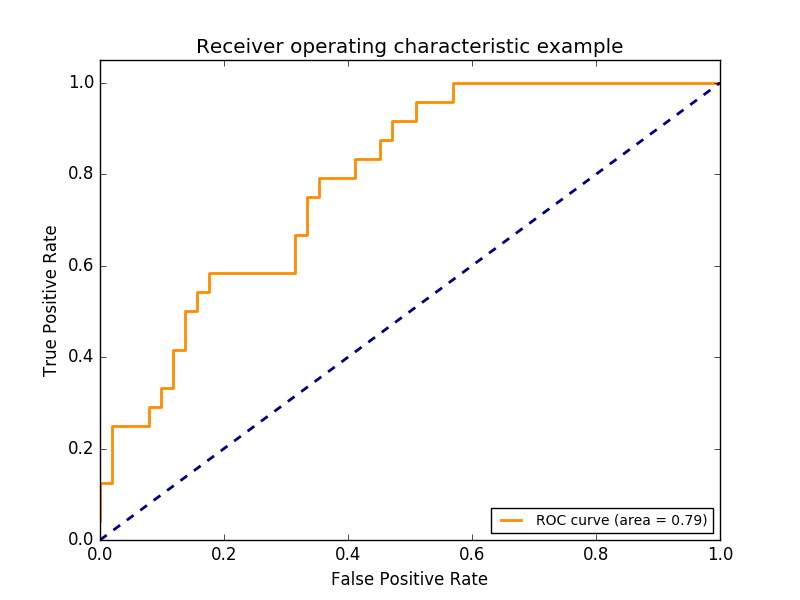
\includegraphics[scale=0.3]{example_roc_1.png}
\end{center}
\end{column}
\begin{column}{5cm}
\begin{center}
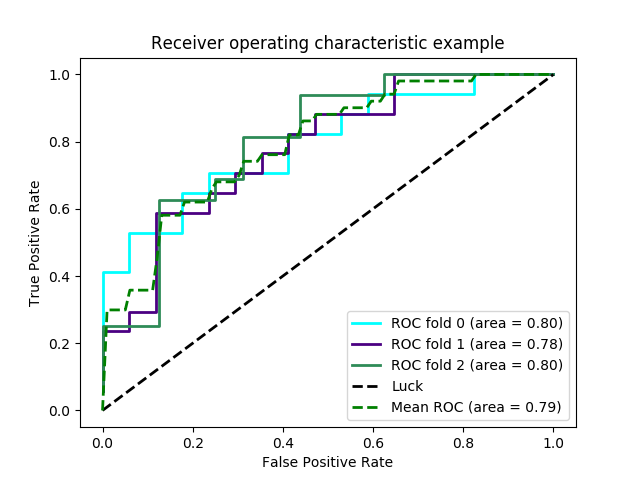
\includegraphics[scale=0.35]{example_roc.png}
\end{center}
\end{column}
\end{columns}
\end{frame}

%%%%%%%%%%%%%%%%%%%%%%%%%%%%%%%%%%%%%%%%%%%%%%%%%%%%%%%%%%%%%%%%%%%%%%%%%%%%%%%%
\begin{frame}[fragile]
\frametitle{Logistic Regression}

\begin{code}
import sklearn.linear_model as lm
help(lm.LogisticRegression)
\end{code}
\end{frame}

%%%%%%%%%%%%%%%%%%%%%%%%%%%%%%%%%%%%%%%%%%%%%%%%%%%%%%%%%%%%%%%%%%%%%%%%%%%%%%%
\frame{   
\frametitle{Objectives}
\begin{block}{}
 \begin{itemize}
  \item[\checkmark] Review
  \item[\checkmark] The sigmoid function
  \item[\checkmark] Logistic regression
  \item[\checkmark] Validation / Confusion Matrix
  \item[\checkmark] ROC Curve
 \end{itemize}
\end{block}
}

%%%%%%%%%%%%%%%%%%%%%%%%%%%%%%%%%%%%%%%%%%%%%%%%%%%%%%%%%%%%%%%%%%%%%%%%%%%%%%%%%%%%%%%%%%
%\section{References}
%%%%%%%%%%%%%%%%%%%%%%%%%%%%%%%%%%%%%%%%%%%%%%%%%%%%%%%%%%%%%%%%%%%%%%%%%%%%%%%%%%%%%%%%%%


%%%%%%%%%%%%%%%%%%%%%%%%%%%%%%%%%%%%%%%%%%%%%%%%%%%%%%%%%%%%%%%%%%%%%%%%%%%%%%%
%\begingroup
\renewcommand{\section}[2]{}%
\frame[allowframebreaks]{
\frametitle{References}
\begin{tiny} \bibliography{../../galvanize.bib}
\bibliographystyle{apalike}         % Style BST file
\end{tiny}
}


\end{document}